\documentclass[12pt]{article}

\usepackage{sbc-template}
\usepackage{graphicx,url}

\usepackage[brazil]{babel}   
%\usepackage[latin1]{inputenc}  
\usepackage[utf8]{inputenc}  
% UTF-8 encoding is recommended by ShareLaTex




\title{\Large Algoritmos e Estrutura de Dados II\\Jogo de 20 Perguntas}%título do artigo
%a palavra Large significa que é para pegar a linha inteira

\author{Antônio Frederico\inst{1},Jefferson Pelinson\inst{1},Joana D’arc P. Barbosa\inst{1}Túlio Faria\inst{1}
	\\Departamento de Ciência da Computação – Instituto Federal de Ciência e Tecnologia\\
	do Sudeste de Minas Gerais - Campus Rio Pomba (IFSEMG)
	\\
	Av. Dr. José Sebastião da Paixão s/no -- Bairro Lindo Vale -- CEP 36180-000\\
	Rio Pomba -- MG -- Brasil
}
\begin{document}%Inicio do documento
	


\section{Introdução}
	
trabalho foi desenvolvido um programa que se utiliza de uma árvore binária para representar uma base de conhecimento.No programa implementamos um jogo chamado "Jogo de 20 Perguntas".O programa interage com o usuário criando uma árvore de perguntas e respostas.No começo do jogo, o jogador inicia a rodada pensando em alguma coisa e em seguida o computador tenta adivinhar o que o usuário pensou. 
\par O computador faz perguntas ao usuário guardando as informações que ele recebe,com estas perguntas ele da um palpite para o usuário tentando adivinhar o que ele pensou,caso esteja certo o computador ganha o jogo.A cada rodada o computador utiliza as informações dos jogos anteriores e ganha mais conhecimento,para isso tivemos que guardar as informações em um arquivo para que elas não fossem perdidas.O usuário é responsável por informar se o computador deve ou não usar essas informações.
\par O programa foi desenvolvido na linguagem Python,por possuir estruturas de alto nível,como as listas ligadas que tem a mesma construção de uma árvore pelo uso de células,pois uma árvore binária também possui uma célula auxiliar que referencia outras duas células,chamadas sub-árvores esquerda e direita.Neste programa a sub-árvore esquerda representa "verdadeiro" e a sub-árvore direita representa "falso",passos que o computador acompanha após as respostas do usuário. 
\newpage
\section{Implementaçâo}
Buscou-se,neste trabalho,implementar um programa chamado ,Jogo de 20 Perguntas.Inicialmente,foi criado uma classe chamada Arvore que tem como parâmetro os nós esquerda e direita da arvore,e também foi adicionado uma variável chamada conteúdo,que representa as informações contidas dentro dos nós.
\begin{figure}[ht]
		\centering
		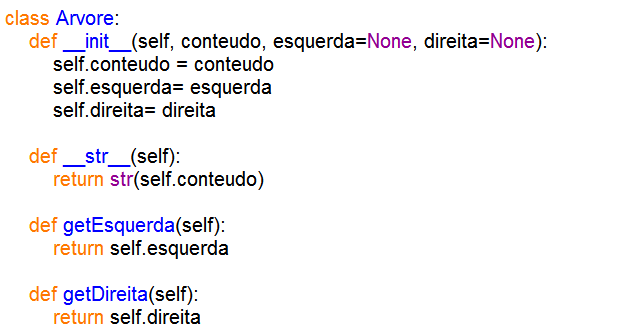
\includegraphics[width=.8\textwidth]{figura1.png}
		\caption{}
\end{figure}
\par O programa também contém uma função chamada verdadeiro,usada durante o funcionamento do jogo ,quando o usuário digita Sim para alguma pergunta ela devolve um valor verdadeiro.
\begin{figure}[ht]
		\centering
		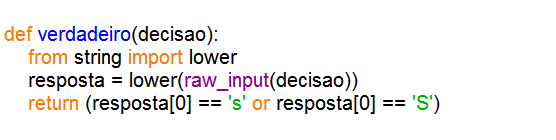
\includegraphics[width=.5\textwidth]{figura2.png}
		\caption{
		}
\end{figure}
\newpage
\par A função principal do programa,chamada main inicia interagindo com o usuário e fazendo a primeira pergunta,a partir da resposta do usuário o laço while caminha pela árvore de cima para baixo.A condição do laço é 'continuar',isso significa que o programa continuará rodando até que o usuário não esteja pensando em nada,ou seja,até que encontre o comando break.
	\begin{figure}[ht]
		\centering
		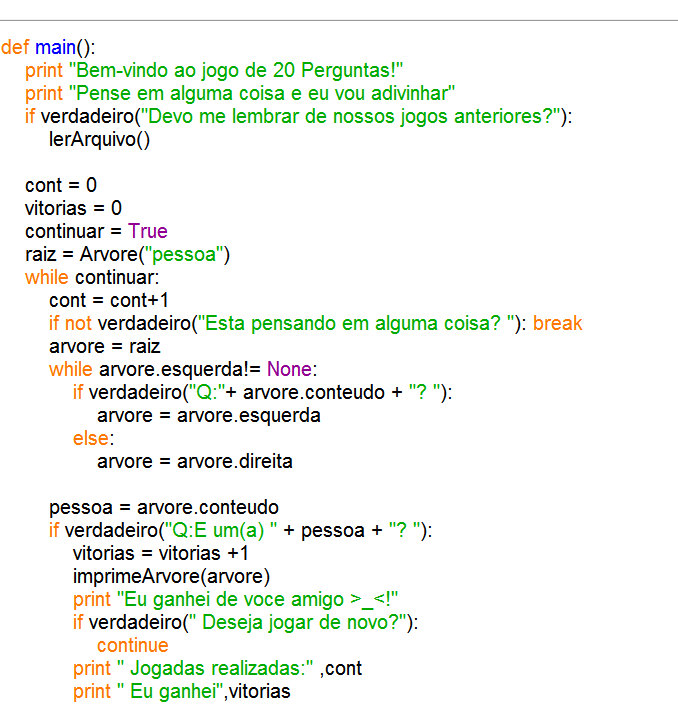
\includegraphics[width=.5\textwidth]{figura3.png}
		\caption{
		}
	\end{figure}
	\newpage
	\par A cada jogada que o usuário faz,o computador guarda as informações obtidas nas jogadas anteriores e as adiciona á árvore.
	\begin{figure}[ht]
		\centering
		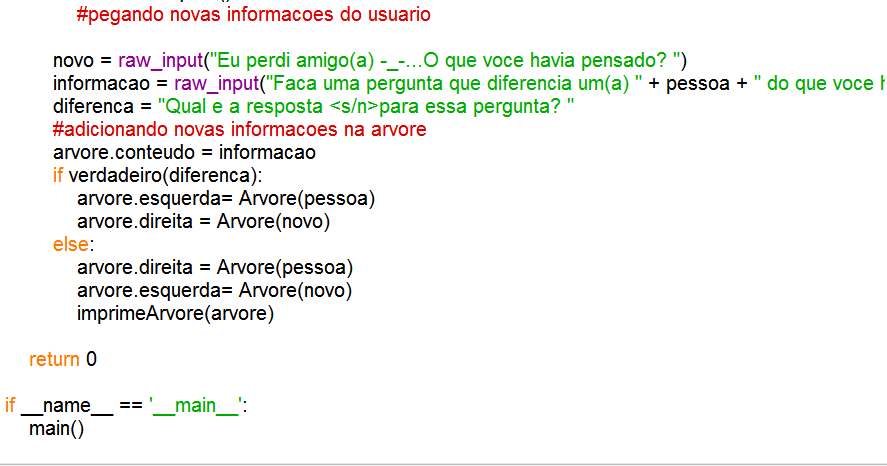
\includegraphics[width=.5\textwidth]{figura4.png}
		\caption{}
		
	\end{figure}
	\newpage
\section{Testes Executados}
Neste capítulo,serão apresentado os testes executados durante o desenvolvimento do programa.
	\begin{figure}[ht]
		\centering
		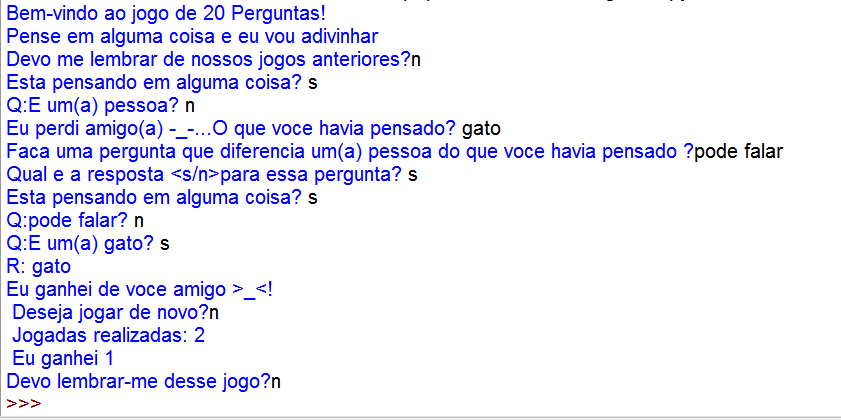
\includegraphics[width=.5\textwidth]{fig0.png}
		\caption{
		}
	\end{figure}
	
	\begin{figure}[ht]
		\centering
		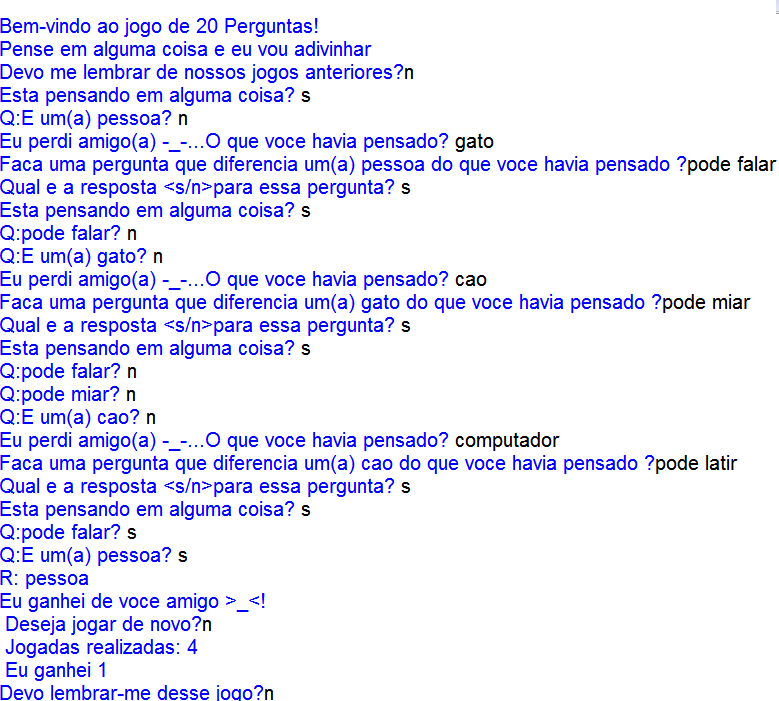
\includegraphics[width=.5\textwidth]{fig1.png}
		\caption{
		}
	\end{figure}
	\begin{figure}[ht]
		\centering
		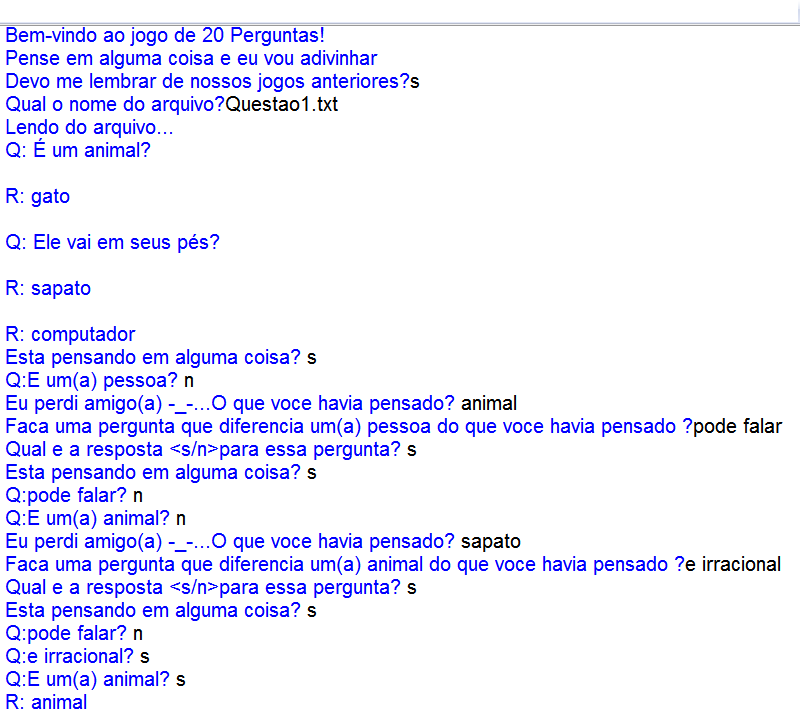
\includegraphics[width=.5\textwidth]{fig2.png}
		\caption{
		}
	\end{figure}
	\begin{figure}[ht]
		\centering
		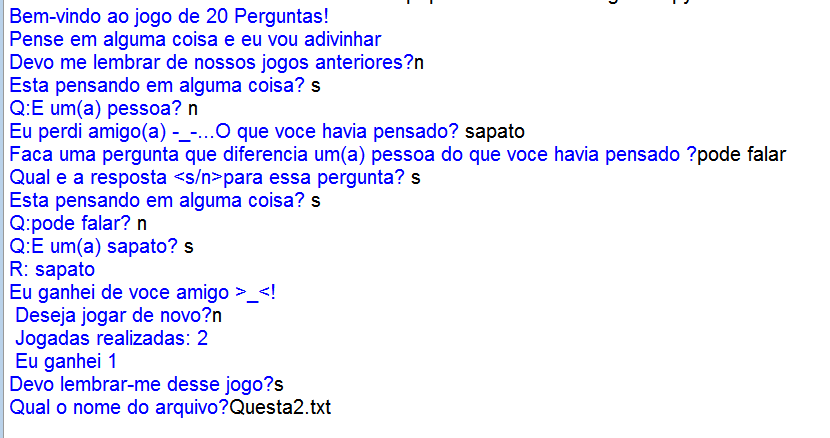
\includegraphics[width=.5\textwidth]{fig3.png}
		\caption{
		}
	\end{figure}
	
	
	
	\newpage
\section{Conclusão}
Este  trabalho teve como objetivo a implementação do Jogo de 20 Perguntas na linguagem Python.
\par O algoritmo do jogo é constituído por uma estrutura de árvore binária e nó (sim e não). Uma função para verificar se a resposta do usuário é um nó sim ou um nó não, este decide para qual direção o algoritmo deverá seguir. Outras funções utilizadas foram para gerar os logs de saída e a entrada de dados externos.
\par Durante o desenvolvimento do trabalho, as maiores dificuldades enfrentadas pelo grupo ao implementar o algoritmo, foram manipular arquivos de entrada/saída e armazenar externamente o estado da árvore binária, uma vez que exigia percorrer a árvore em ordem correta para obtenção das perguntas e respostas em sua respectiva sequência.
\par Concluímos que o desenvolvimento deste trabalho foi de grande importância para nossa compreensão e aprofundamento do tema abordado, pois visto que nos permitiu desenvolver um jogo interativo utilizando-se dos conhecimentos adquiridos nas aulas.
	
\newpage
\begin{thebibliography}{1}
		
		\bibitem {DOWNEY et.al}DOWNEY,A., ELKNER,J., MEYERS,C.
		\textbf{\textit{Como pensar como um Ciêntista da Computação usando Python.}}janeiro 2008.
		\bibitem {BORGES}BORGES,L.E.
		\textbf{\textit{Python para Desenvolvedores.}}
		2 edição.
		
		
\end{thebibliography}%fim das referencias
\thispagestyle{empty}
\end{document}%fim do documento

